% Appendix B
 
\chapter{Designing Figures and Tables}
\label{cha:designingfigtab}
\label{appendixb}

In Section~\ref{sec:tablesfigureslistings}, we have shown how you can integrate tables, figures, and listings into your thesis. In this appendix, we give recommendations on a higher level. In the following sections, we focus on \emph{designing} compelling figures and tables, i.\,e., how you can present material effectively. For figures, we will cover both graphs as well as diagrams.

We\marginnote{While this guide is published under a Creative Commons license (cf. Sect.~\ref{sec:license}), this license does not apply to the reproduced figures. Elsevier and/or the authors hold the copyright for the reproduced figures.}
have compiled most of the content in this appendix from the following two books (permission to reproduce the respective figures has been obtained from Elsevier):
\begin{itemize}
  \item the book \emph{Designing Science Presentations: A Visual Guide to Figures, Papers, Slides, Posters, and More} by Matt Carter, © 2012 \cite{Carter12} and
  \item the book \emph{Information Visualization: Perception for Design} by Colin Ware, © 2012 \cite{Ware12}.
\end{itemize}

Another useful resource is the book \emph{Universal Principles of Design: 125 Ways to Enhance Usability, Influence Perception, Increase Appeal, Make Better Design Decisions, and Teach Through Design} \cite{Lidwell10}.
  
\section{Fundamental Concepts}

We start by revisiting the fundamentals of visual perception as well as information organization. The following section will apply the concepts shown in this section.

When you design figures, you should be aware of the Gestalt laws and the HSB color model, which will be described in the following two sections. After that, we will revisit the basics of information organization, which apply to figures and tables alike.

\subsection{Gestalt Laws}

The Gestalt laws have been known since the early 1900s. They describe how we perceive patterns. In the following, we will discuss the following Gestalt laws: proximity, similarity, connectedness, continuity, symmetry, closure, and relative size.

\begin{marginfigure}
\centering
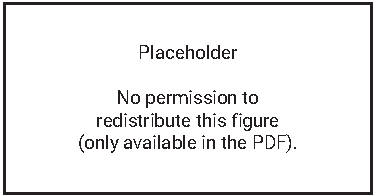
\includegraphics[width=1\textwidth]{gestalt-proximity}
\caption{\label{fig:proxi} Spacing makes us perceive rows or columns (reproduced from \cite{Ware12} with permission).}%[-1\baselineskip]
\end{marginfigure}


The first law, \textbf{proximity}, refers to the spatial relationships between groups of objects. Objects that are closer together form a group. We are very sensitive to spatial relationships. Even small changes in spacing can change our interpretation of a scene (cf. Fig.~\ref{fig:proxi}). Therefore, you should ``place symbols and glyphs representing related information close together.'' 
\cite{Ware12}. The proximity law is the reason why adding additional vertical space between (groups of) rows helps us with reading a table.

\begin{marginfigure}[-2\baselineskip]
\centering
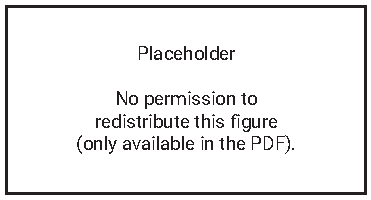
\includegraphics[width=1\textwidth]{gestalt-similarity}
\caption{\label{fig:simi} We perceive similar elements as a group (reproduced from \cite{Ware12} with permission).}
\end{marginfigure}

\textbf{Similarity} is the second Gestalt law. Visual similarities such as color or shape allow us to identify groups of objects with ease (cf. Fig.~\ref{fig:simi}). Large tables, for instance, can benefit from alternated shading of rows. A downside of shading is the additional visual clutter. We prefer to add extra space every three to five rows to keep tables readable. The similarity law is also essential in diagrams that use different shapes or styles. Visual differences help the reader group similar elements.


\textbf{Connectedness} is a powerful principle that is stronger than proximity, shape, and style (cf. Fig.~\ref{fig:connectedness}). Consider connecting related objects with lines.
\begin{marginfigure}[-2\baselineskip]
\centering
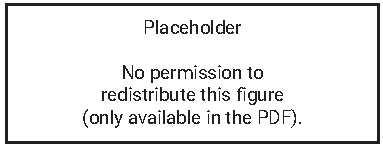
\includegraphics[width=1\textwidth]{gestalt-connectedness}
\caption{\label{fig:connectedness} Connections are more powerful than similarity (reproduced from \cite{Ware12} with permission).}
\end{marginfigure}

The next principle, \textbf{continuity}, ``states that we are more likely to construct visual entities out of visual elements that are smooth and continuous, rather than ones that contain abrupt changes in direction'' \cite{Ware12}. It is, therefore, not surprising that node-link diagrams with smooth lines are easier to read than those with straight lines (cf. Fig.~\ref{fig:continuity}).

\begin{marginfigure}[-1\baselineskip]
\centering
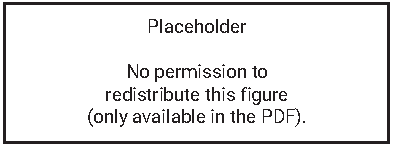
\includegraphics[width=1\textwidth]{gestalt-continuity}
\caption{\label{fig:continuity} Continuity makes the left-hand diagram easier to read (reproduced from \cite{Ware12} with permission).}
\end{marginfigure}

\begin{figure}
\centering
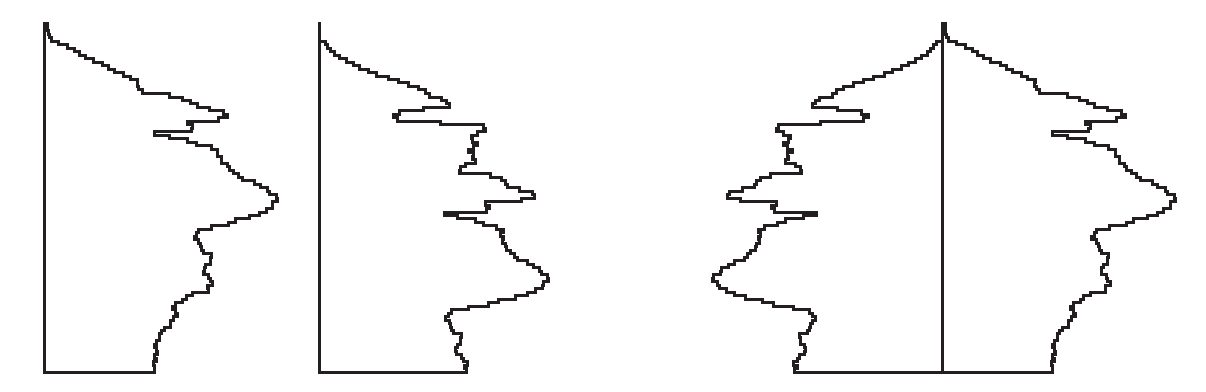
\includegraphics[width=1\textwidth]{gestalt-symmetry}
\sidecaption{\label{fig:symmetry} We can spot differences in these age distribution plots faster when data is plotted symmetrically (Data source: \url{https://destatis.de}, own illustration).}[-6\baselineskip]
\end{figure}

Another principle is \textbf{symmetry}. Symmetrical figures are visually pleasing, and we are good at detecting asymmetry. Symmetry is a form of high-level similarity. If you organize groups of elements in a diagram symmetrically, readers will assume that this means that they are similar. If you design diagrams asymmetrically, the asymmetric parts get emphasized. Our ability to check for symmetry can also be useful during visual data analysis (cf. Fig.~\ref{fig:symmetry}).

\begin{marginfigure}
\centering
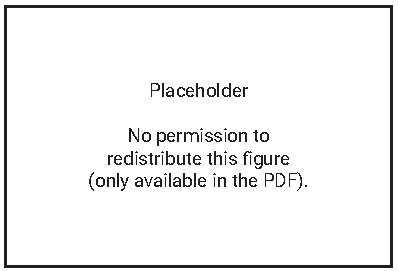
\includegraphics[width=1\textwidth]{gestalt-closure}
\caption{\label{fig:closure} Left: closure makes us perceive a full circle (reproduced from \cite{Ware12} with permission); right: the orange dot is perceived to sit inside of a rectangle.}
\end{marginfigure}

We are also on the lookout for \textbf{closure and common ground}. Closed contours are perceived as objects. Our search for closure is so strong that our brain interpolates missing parts of contours to form whole objects. As a result, we see a rectangle and a complete circle on the left-hand side of Fig.~\ref{fig:closure} instead of a circle with a missing segment. Moreover, contours create a notion of common ground with an ``inside'' and an ``outside''.

Common grounds are perceived for complete contours as well as for contours that we perceive due to closure. Thus, on the right-hand side of Fig.~\ref{fig:closure}, we perceive the orange dot to be inside an imaginary rectangle built by shapes. Ware recommends: ``Consider putting related information inside a closed contour. A line is adequate for regions having a simple shape. Color or texture can be used to define regions that have more complex shapes'' \cite{Ware12}.

The final Gestalt law to discuss is \textbf{figure and ground}. Figures are perceived as objects that are positioned in the foreground. The ground lies behind the figures. We perceive an object as a figure when it consists of a closed contour that forms a common ground and is considerably smaller compared to its surroundings.

\begin{marginfigure}
\centering
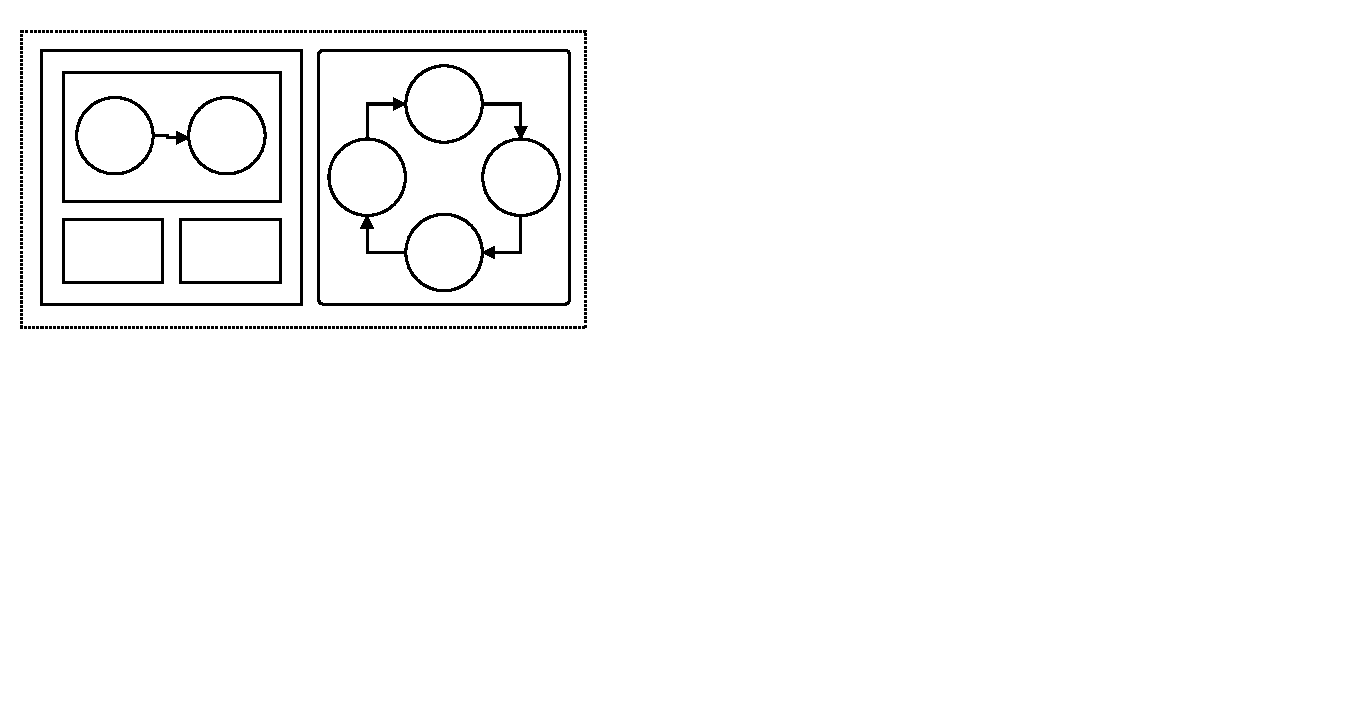
\includegraphics[width=1\textwidth]{gestalt-figureground}
\caption{\label{fig:figureground} Figure and ground are difficult to pick apart in this diagram; also note how PowerPoint fails to draw straight connectors (own illustration).}%[-1\baselineskip]
\end{marginfigure}

This principle is important when drawing diagrams that use contours to demarcate the boundaries of various systems. When multiple systems are nested, and the size differences are too small, it can become difficult to perceive the difference between figure and ground. Consider the diagram shown in Fig.~\ref{fig:figureground}). On the left-hand side of this diagram, too many rectangular shapes have been nested. Due to equal amounts of whitespace around every shape, multiple interpretations are possible. The right-hand side of the diagram is slightly better because the circles are considerably smaller than the surrounding rectangle. Moreover, together with the arrows the circles are perceived as a (symmetric) shape, which is easily perceived as a figure sitting on the rectangle in the background.


% Gestalt Theory and Instructional Design , Moore and Fitz 1993
% http://citeseerx.ist.psu.edu/viewdoc/download?doi=10.1.1.1026.6390&rep=rep1&type=pdf


\subsection{Color}
\label{sec:color}

You are probably used to defining colors in terms of red, green, and blue (RGB) or cyan, magenta, yellow, and black (CMYK). A third way, which is more useful, is the \textbf{HSB model}. It defines color in terms of hue, saturation, and brightness.\sidenote{Read the primer at \url{https://learnui.design/blog/the-hsb-color-system-practicioners-primer.html} for more details.} Consider the color picker shown in Fig.~\ref{fig:hsb} for an example.

\begin{figure}
\centering
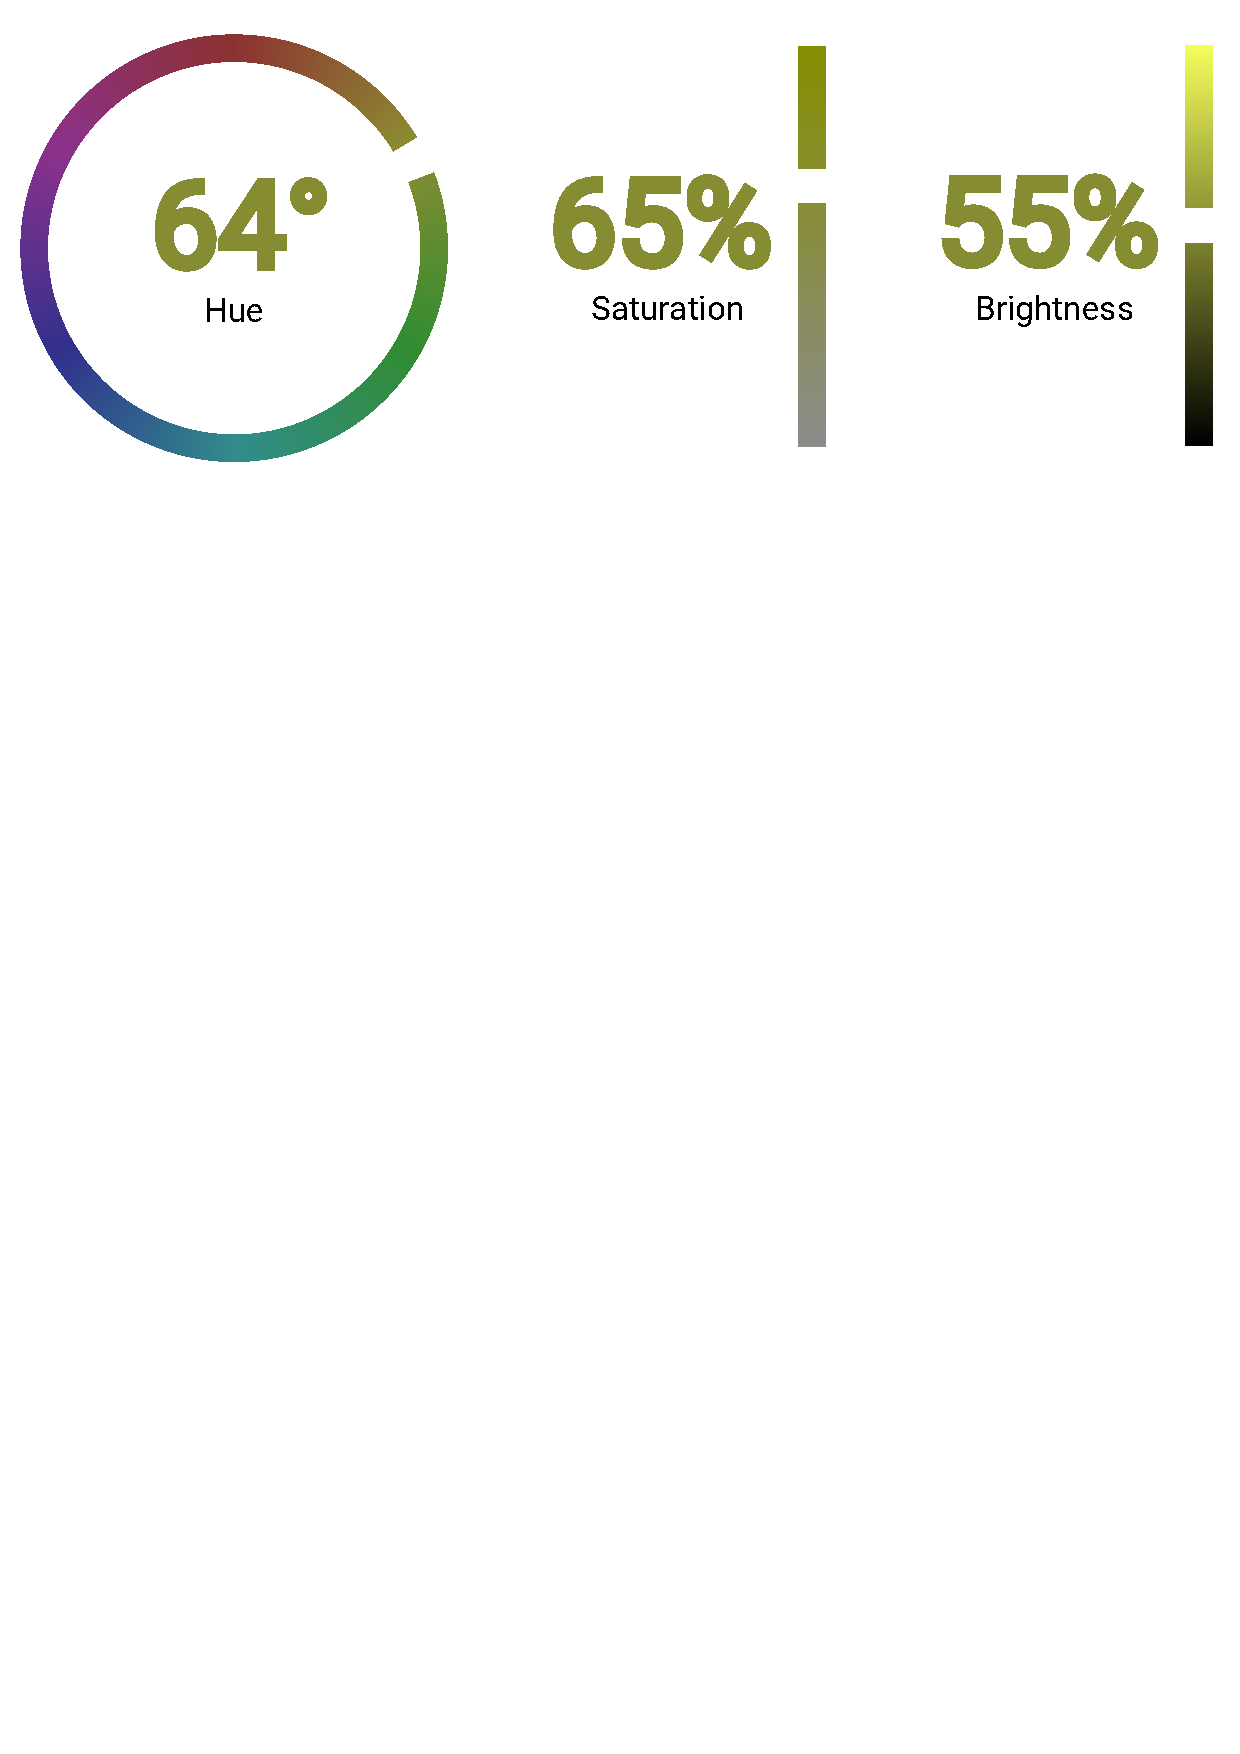
\includegraphics[width=0.85\textwidth]{color-hsb}
\sidecaption{\label{fig:hsb} A HSB color picker (\url{https://codepen.io/HunorMarton/full/eWvewo})}[-2\baselineskip]
\end{figure}

The first value, \textbf{hue}, defines the color according to its position (given in degrees ranging from 0 to 360) on the color wheel. For instance, the value of 60 corresponds to the hue yellow. \textbf{Saturation} (0 to 100) corresponds to the richness of the color, where 0 means that there is no trace of the hue, i.\,e., a gray color between white and black. The value 100 means that the hue is fully present, i.\,e., the color is as colorful as possible. The final value is \textbf{brightness} (0 to 100). A value of 0 corresponds to a solid black, a value of 100 corresponds to the brightest version of the hue at the given saturation.

\begin{marginfigure}
\centering
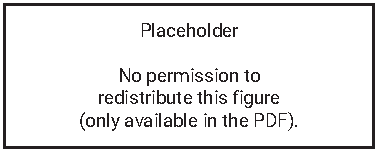
\includegraphics[width=1\textwidth]{color-plots}
\caption{\label{fig:coloredgraphs} Using colors to ease visual perception (reproduced from \cite{Carter12} with permission).}%[-1\baselineskip]
\end{marginfigure}

Different colors are often used to ease visual perception (cf. Fig.~\ref{fig:coloredgraphs}). For instance, it can be used for emphasis, to group subsets of elements, or to make it easier to distinguish different elements that have a similar shape.

Be aware of the monochrome representation of colors, which makes it impossible to distinguish a subset of colors. Red and green are particularly difficult to differentiate in monochrome print, especially if they have the same saturation and brightness (cf. Fig.~\ref{fig:monochrome}).

\begin{marginfigure}[-5\baselineskip]
\centering
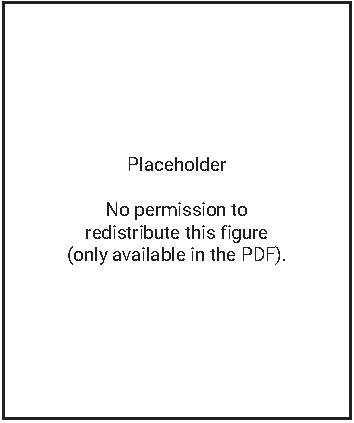
\includegraphics[width=0.8\textwidth]{color-mono}
\caption{\label{fig:monochrome} Colors in monochrome (reproduced from \cite{Carter12} with permission).}
\end{marginfigure}

The risk of confusion in monochrome prints is not the only reason why changing the hue is problematic. Different hues are difficult to make out when the area is small, as in the line plot in  Fig.~\ref{fig:coloredgraphs}. Moreover, different colors (hues) have different connotations (such as green means good, red means danger). Finally, different colors have a different visual weight that may create unwanted emphasis (blue is heavier than orange).

Therefore, it is often better to stick with one hue and use different levels of brightness or saturation to ease visual perception. Figure~\ref{fig:monographs} uses three shades of gray and is easier to read than the colorful version in Fig.~\ref{fig:coloredgraphs}.


\begin{marginfigure}
\centering
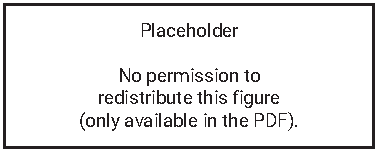
\includegraphics[width=1\textwidth]{color-plots-mono}
\caption{\label{fig:monographs} Shades of gray can be very effective (reproduced from \cite{Carter12} with permission).}%[-1\baselineskip]
\end{marginfigure}

When you use more than four different grayscale colors, however, the differences become too small to perceive with ease. Too many grayscale colors are especially problematic when color is used on its own, such as in line plots. It is less problematic in bar plots, because the bars can be sorted with decreasing brightness levels to create (good) redundancy. If brightness is used to encode values of data, darker colors should be used for higher values.

Similar principles apply for saturation: ``If using color saturation to encode numerical quantity, use greater saturation to represent greater numerical quantities. Avoid using a saturation sequence to encode more than three values'' \cite{Ware12}. Consider varying both brightness and saturation at the same time to create shades that are easier to distinguish from another.

\begin{marginfigure}
\centering
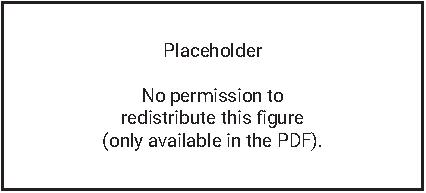
\includegraphics[width=1\textwidth]{color-saturation}
\caption{\label{fig:saturation} Use less saturation for large shapes, and more for thin lines (reproduced from \cite{Ware12} with permission).}%[-2\baselineskip]
\end{marginfigure}

The effects of different levels of saturation vary depending on the size of the colored area (cf. Fig.~\ref{fig:saturation}). If you consider varying saturation, stick to the following guidelines: ``Use more saturated colors when color coding small symbols, thin lines, or other small areas. Use less saturated colors for coding large areas'' \cite{Ware12}.


\section{Organizing Information}
\label{sec:organizinginfo}

In this section, we will review selected design concepts to organize information in a meaningful way. The book by Lidwell et al. contains more information on the ideas \cite{Lidwell10}.

\subsection{Advance Organizer}

An often-cited principle for giving a speech is summarized as follows: first, you announce what you are going to talk about; second, you talk about that; third, you review what you talked about. A design concept that implements this advice is an \emph{advance organizer}. Advance organizers are short chunks of information that are presented before new material. This way, readers will find it easier to learn new concepts.

Note that an advance organizer is not just a summary or an abstract. Its purpose is to relate new pieces of information to previously covered material and explain how this fits into the big picture. There are two kinds of advance organizers: expository and comparative.

\emph{Expository advance organizers}, as Lidwell et al. \cite{Lidwell10} explain, ``are useful when audiences have little or no knowledge similar to the information being taught.'' Expository advance organizers are effective when they provide a concise overview of the new material and how it fits together and into the big picture.

On the other hand, \emph{comparative advance organizers} ``are useful when audiences have existing knowledge similar to the information being presented. [They] compare and contrast features and operations between the familiar and the new'' \cite{Lidwell10}.

You can create advance organizers in the form of diagrams or as plain text. As a first step, you can add a \emph{signpost paragraph} at the beginning of chapters and sections.

\subsection{Hierarchy}

Complicated relationships are often explained using a hierarchical approach. 
There are three basic ways to represent hierarchy: trees, nests, and stairs (cf. Fig.~\ref{fig:hierarchy}).


\begin{marginfigure}
\centering
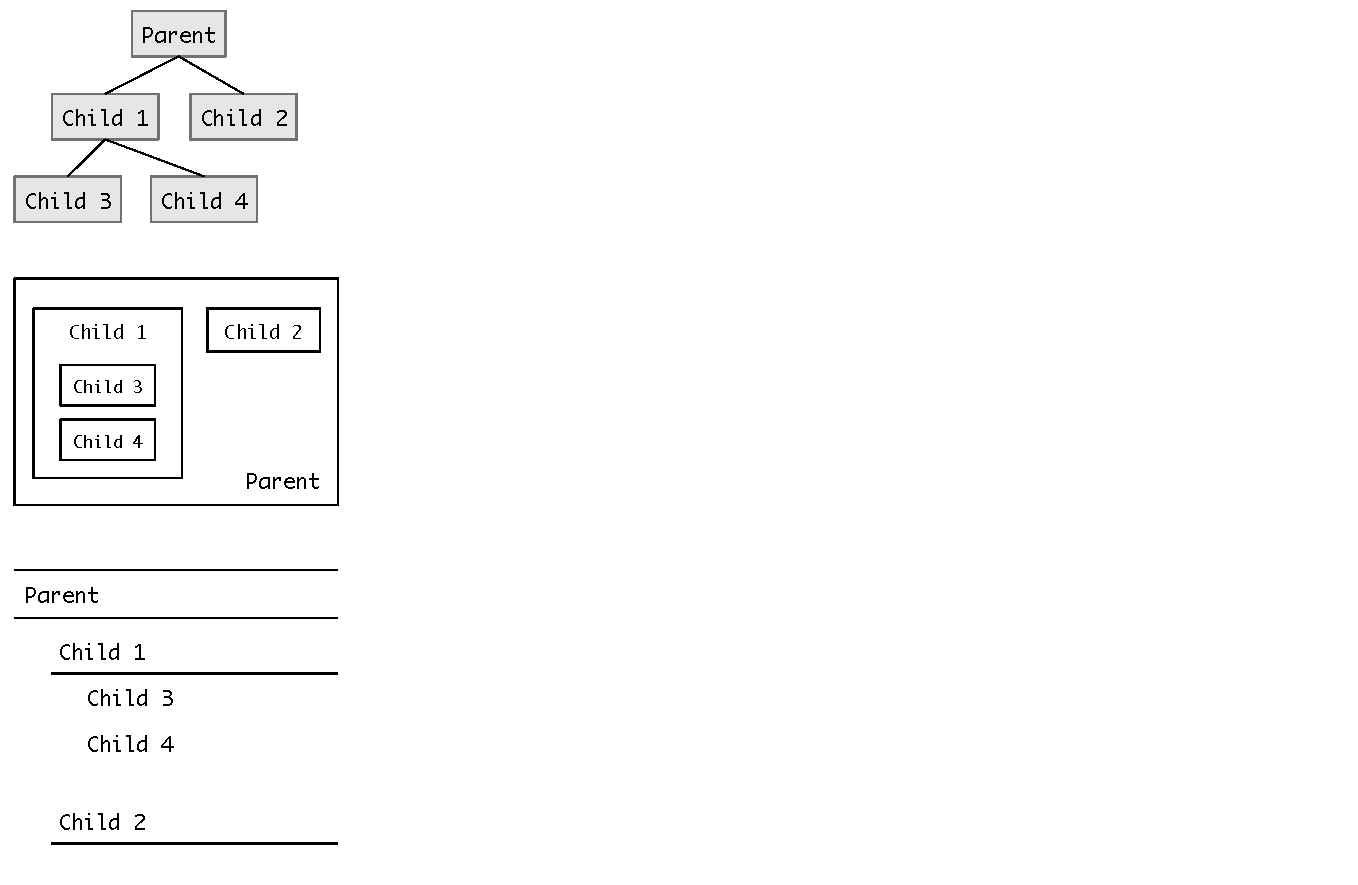
\includegraphics[width=1\textwidth]{info-orga-hierarchy}
\caption{\label{fig:hierarchy} You can visualize hierarchies with trees, nests, and stairs (own illustration).}%\cite{Lidwell10}.} 
\end{marginfigure}


\emph{Trees} are useful to visualize structures that consist of parent-child relationships such as A dominates B and C, B dominates of D and E, and so on. 
Usually, child elements are located below or to the right of their parents. As Lidwell et al. \cite{Lidwell10} observe, ``tree structures grow large quickly, and become tangled when multiple parents share common child elements. Tree structures are commonly used to represent overviews or high-level maps of system organization.''

\emph{Nest visualizations} are especially useful in visualizing parent elements that \emph{contain} child elements. Nest visualizations can be challenging to read when relationships are complicated.

Finally, \emph{stair structures} stack child elements below and to the right of parent elements. Stair visualizations are common in outlines. They can be used to capture arbitrarily complex hierarchies, especially when used interactively and individual nodes can be collapsed. Stair visualization also has a disadvantage: it may falsely imply a sequential relationship between the stacked child elements.

\subsection{Five Ways of Organization}
\label{sec:fivehatracks}

The so-called \emph{Five Hat Racks} design principle suggests five common ways to organize information: by category, time, location, alphabet, and continuum \cite{Lidwell10}.

\begin{enumerate}
\item \textbf{Organization by category} relies on similarity or relatedness of elements. Sometimes, categories can be organized hierarchically fashion.Note, Category is a nominal attribute, i.\,e., there is no natural order. If categories \emph{have} to be ordered, you can rely on alphabetical order or use an apparent order such as ``start with all the \emph{normal} categories, followed by the special ones.''

\item \textbf{Organization by time} is based on some chronological sequence. Ordering by time feels very natural. Note, however, that a chronological organization is not always useful. A literature review that merely presents one paper after another chronologically will not generate much insight.

\item \textbf{Organization by location} relies on geographical or spatial properties of the elements. Location can also be purely a logical concept, for instance, components that make up a system (which is also a hierarchy). It is common to describe systems by explaining one component (location) after another.

\item \textbf{Alphabetical organization} is another common technique. As Lidwell et al. \cite{Lidwell10} remark, ``organize information alphabetically, when information is referential, when efficient nonlinear access to specific items is required, or when no other organizing strategy is appropriate.''

\item \textbf{Organization by continuum} relies on a numeric property of the elements (e.\,g., ordering from highest to lowest or best to worst). Lidwell et al. \cite{Lidwell10} recommend to ``organize information by continuum when comparing things across a common measure.'' Organization by continuum can improve the readability of bar plots (cf. Fig.~\ref{fig:continuum})
\end{enumerate}


\begin{marginfigure}
\centering
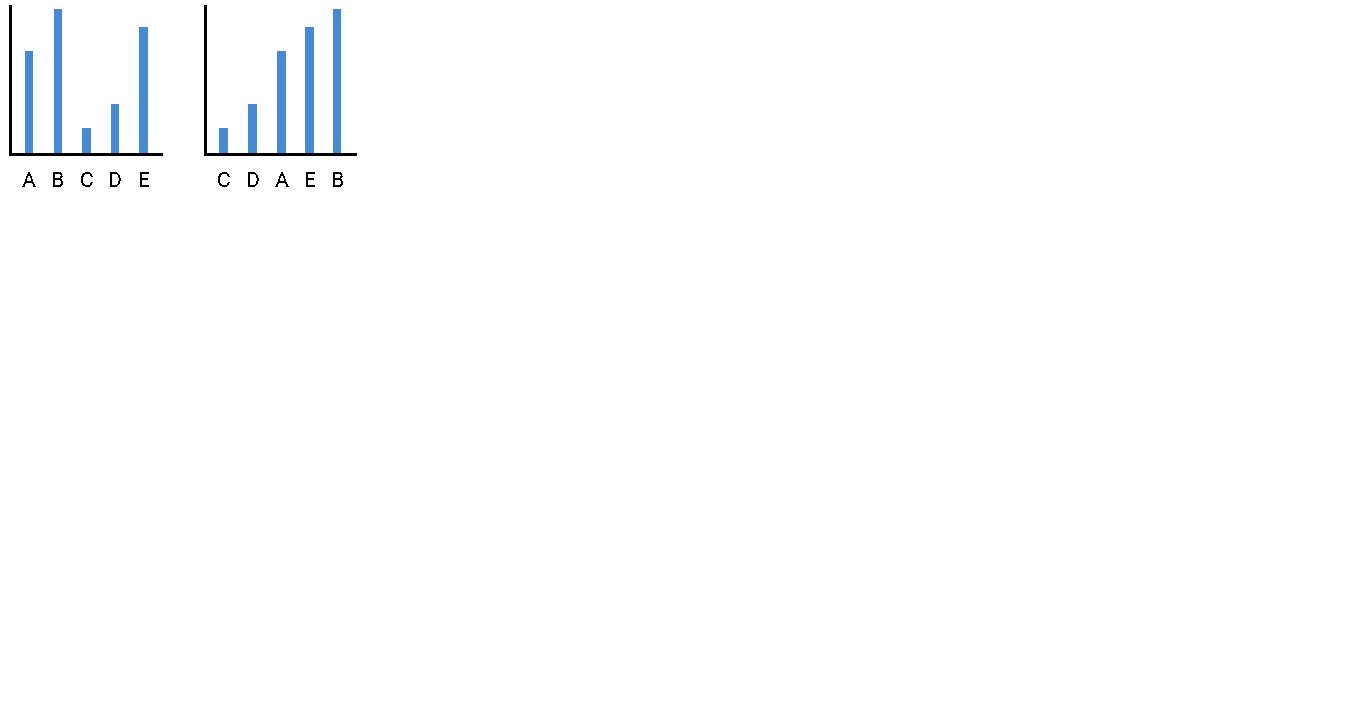
\includegraphics[width=1\textwidth]{info-orga-continuum}
\caption{\label{fig:continuum} Bar plots benefit from ordering the bars by length, an application of organization by continuum (own illustration).}%\cite{Lidwell10}.} 
\end{marginfigure}


\section{Diagrams}

You can use diagrams to describe concepts and their relationship, the structure of systems, interactions, and (experimental) procedures.

%\subsection{Common Problems}
% infohq
% examples

\subsection{Before You Start}

Your first task is to decide \emph{whether a visualization makes sense at all}. Sometimes it makes sense to choose a text-only representation such as pseudo-code instead of a diagram. Ware \cite{Ware12} shares the example of a flow chart, which is supposed to make it easier to understand the program flow (cf. Fig.~\ref{fig:flowchart}). He argues that pseudo code is superior. After all, the flow chart takes more effort to parse than the natural language used in the pseudo code (and, as Edward Tufte would argue, the flow chart contains more visual clutter than the pseudo code).

\begin{figure}[t]
\centering
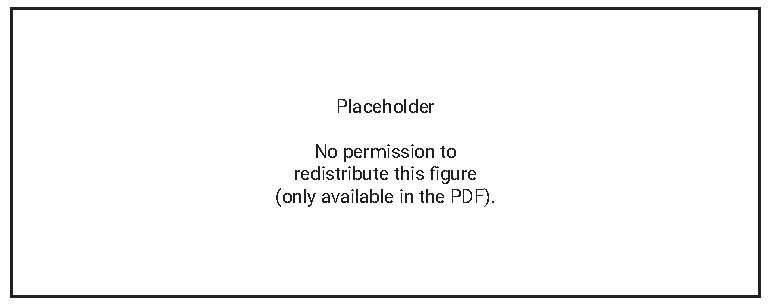
\includegraphics[width=1\textwidth]{diagram-flowchart}
\decoRuleFlex{1\textwidth}
\sidecaption{\label{fig:flowchart} In comparison to pseudo code a flow chart is a poor representation of program flow (reproduced from \cite{Ware12} with permission).}[-6\baselineskip]
\end{figure}

On the other hand, Ware argues, there are concepts that we can grasp much faster if we see a visual representation. Consider the following statements about a management hierarchy \cite{Ware12}:

\begin{itemize}
  \item Jane is Jim’s boss.
  \item Jim is Joe’s boss.
  \item Anne works for Jane.
  \item Mark works for Jim.
  \item Anne is Mary’s boss.
  \item Anne is Mike’s boss
\end{itemize}


\begin{marginfigure}
\centering
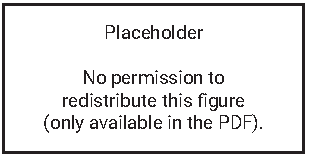
\includegraphics[width=1\textwidth]{diagram-tree}
\caption{\label{fig:tree} A tree helps us grasp static relationships (reproduced from \cite{Ware12} with permission).}%[-2\baselineskip]
\end{marginfigure}

It is challenging to keep track of all relationships in this presentation. You might even feel the urge to draw a tree. And, indeed, a graphical representation is much more accessible (cf. Fig.~\ref{fig:tree}). Ware concludes: ``Diagrams should be used to express structural relationships among program elements, whereas words should be used to express detailed procedural logic'' \cite{Ware12}.


Now, if you decide that you do want to create a diagram, you should ask yourself the following questions \cite{Carter12}:
\begin{itemize}
\item What is absolutely necessary to show?
\item What is not necessary to show?
\item What is most important and should be emphasized?
\item What is not important and should be secondary to the main message?
\item What are the relationships between individual elements?
\item Does the diagram require a precise depiction of time?
\item Does the diagram require a precise depiction of distance?
\item What symbols should be consistent throughout the diagram?
\end{itemize}

In the following sections, we will explain the most important aspects to create useful diagrams.

\subsection{Elements and Relationships}

According to the Gestalt laws, you should
``use small, closed shapes to represent data entities, and use the color, shape, and size of those shapes to represent attributes of those entities'' \cite{Ware12}. Figure~\ref{fig:entities} shows the effect of different properties of shapes.

\begin{figure}[t]
\centering
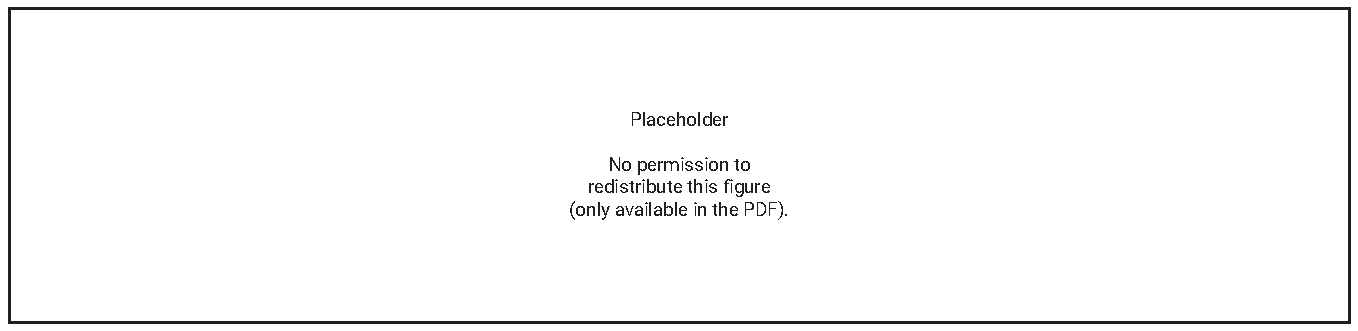
\includegraphics[width=1\textwidth]{diagram-entities}
\sidecaption{\label{fig:entities} Semantics of four properties of shapes (reproduced from \cite{Ware12} with permission).}[-5\baselineskip]
\end{figure}

Many diagrams are supposed to visualize relationships of elements. Ware recommends to use ``connecting lines, enclosure, grouping, and attachment to represent relationships between entities. The shape, color, and thickness of lines and enclosures can represent the types of relationships'' \cite{Ware12}. Figure~\ref{fig:relationships} visualizes ten alternatives and how we perceive them.

Of note are the tapered lines in Number 6 of Fig.~\ref{fig:relationships}. As explained by Ware, these are easier to recognize than arrows \cite{Ware12}, especially in busy diagrams. If you only use straight lines, you can use skinny triangles to create tapered lines. The broad end is located at the source of the line.

For more complex lines, you need a vector drawing tool like Inkscape, Adobe Illustrator, and Affinity Designer. Such tools also allow you to draw the wiggly line shown in Number 7 of Fig.~\ref{fig:relationships}. Most drawing tools enable you to create shapes with receptacles (cf. Number 9 of Fig.~\ref{fig:relationships}) by creating unions and differences of shapes.



\begin{figure}[t]
\centering
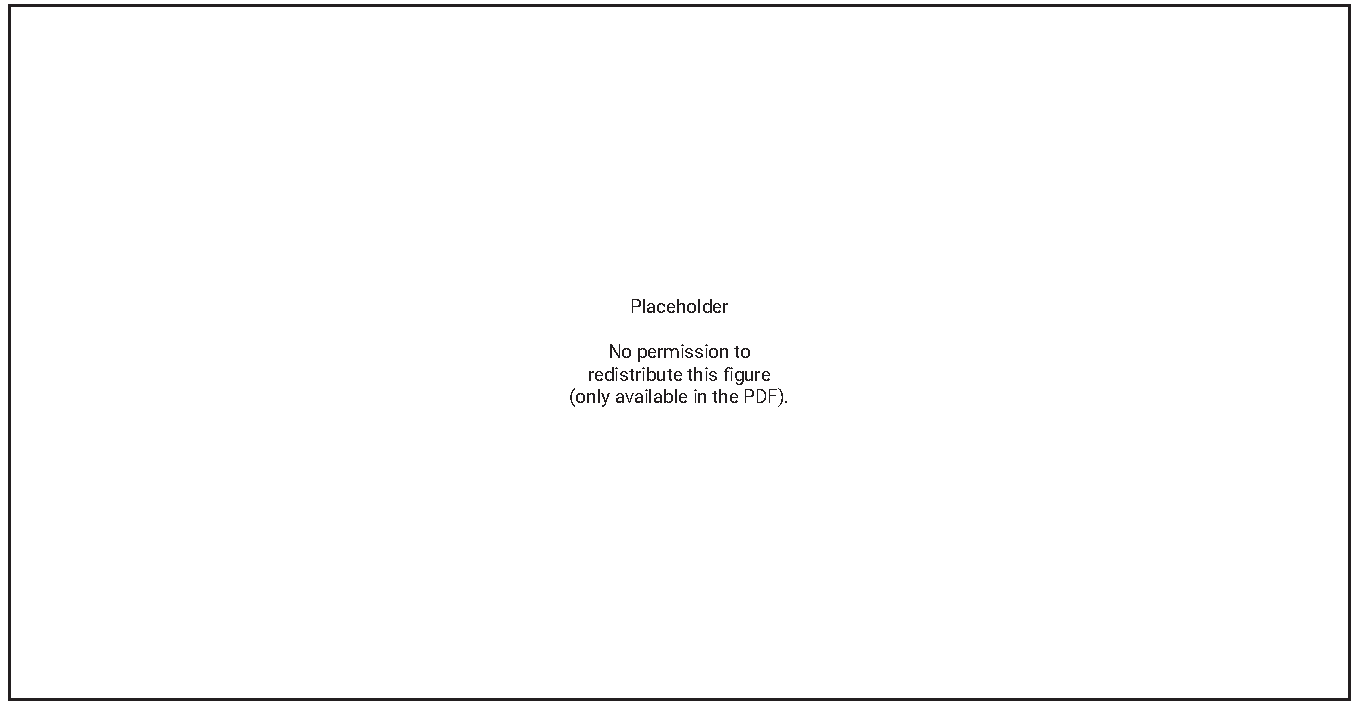
\includegraphics[width=1\textwidth]{diagram-relationships}
\sidecaption{\label{fig:relationships} Semantics of ten types of visual relationships (reproduced from \cite{Ware12} with permission).}[-5\baselineskip]
\end{figure}



\subsection{Emphasizing Elements}

Useful diagrams are self-explanatory and guide the reader's attention. Humans continuously search for patterns and deviations. Consistent use of shapes and colors indicates that the presented elements are similar (cf. Fig.~\ref{fig:emphasis}). Deviations from the norm indicate differences that need attention. Be aware of that, and do not create emphasis unintentionally.

\begin{figure}[t]
\centering
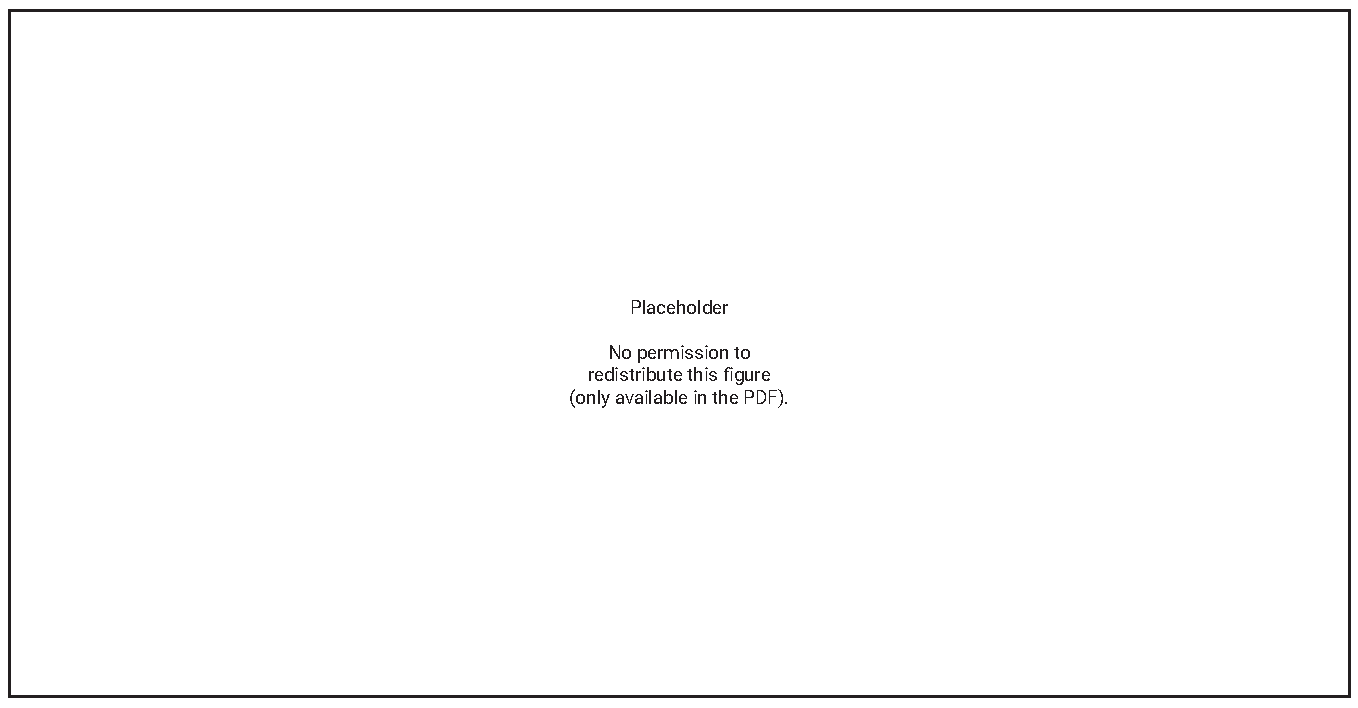
\includegraphics[width=1\textwidth]{diagram-emphasis}
\sidecaption{\label{fig:emphasis} Deviations from the norm create emphasis (reproduced from \cite{Carter12} with permission).}[-6\baselineskip]
\end{figure}

Do not choose the size of elements arbitrarily. Differences translate into dominance relationships. Larger elements usually appear to control the smaller ones (cf. Fig.~\ref{fig:dominance})

\begin{figure}[t]
\centering
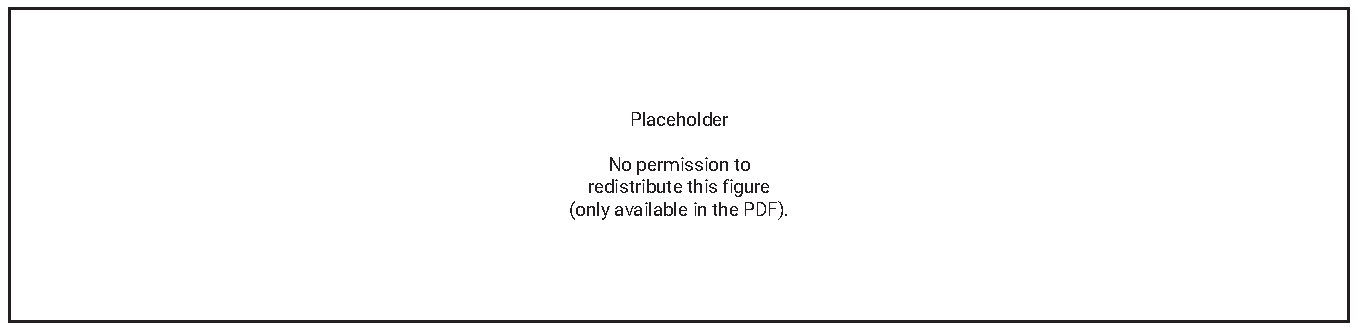
\includegraphics[width=1\textwidth]{diagram-dominance}
\sidecaption{\label{fig:dominance} Relative differences in size indicate dominance relationships (reproduced from \cite{Carter12} with permission).}[-6\baselineskip]
\end{figure}


\subsection{Layout}

In the absence of strong emphasis, readers process diagrams similar to text (cf. Fig.~\ref{fig:direction}). In western cultures, readers will start in the top left corner and proceed horizontally in a zig-zag pattern. The general flow of information should be consistent with this expectation.

\begin{marginfigure}
\centering
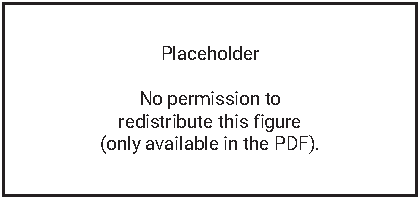
\includegraphics[width=1\textwidth]{diagram-direction}
\caption{\label{fig:direction} Respect the expected flow of information in western cultures (reproduced from \cite{Carter12} with permission).}%[-1\baselineskip]
\end{marginfigure}


Ensure that all elements of a diagram are correctly aligned. Alignment helps readers to grasp the overall structure. Proper alignment can also save you from creating additional outlines to depict (systems) boundaries – proximity and neat alignment can create strong cohesion by themselves (closure).

Make conscious decisions about distances and dimensions (proximity, repetition). You \emph{can} use a \emph{grid} to enforce consistent distances. Note, however, that snapping every element to the grid lines, may \emph{still} cause misalignment.\sidenote{Consider a shape that is five grid lines high. Then, a horizontal line that leaves the box cannot be aligned in the middle.} Make use of the horizontal and vertical alignment tools that space out elements equally. An advanced technique is to create a dummy box shape to measure and compare dimensions yourself.

\subsection{Labels}

Many diagrams consist of shapes and lines, annotated with text labels.

A common technique is to use bold print to express some property of an element. For instance, the labels of shapes corresponding to systems are printed in bold to differentiate them from the shapes that correspond to exchanged messages. In general, we recommend avoiding this practice. Reserve bold print to emphasize \emph{one particular element} in a diagram. Use another visual style to show differences, such as shading, colors, or shape form. Consider giving an element no surrounding shape at all, for instance, if the notion of its \emph{boundary} is not relevant or if the arrangement of sub-elements establishes a common ground due to the Gestalt law of \emph{closure}.

In any case, the labels should be as close as possible to the shapes (Gestalt law proximity) and precisely aligned. Whenever possible, consider moving the labels \emph{into} the shapes (Fig.~\ref{fig:labelsinside}). Inside labels rely on the Gestalt law of \emph{common ground}. They reduce visual clutter and make it easier to create a well-balanced diagram with no ragged edges (laws of symmetry and closure). 

\begin{figure}[t]
\centering
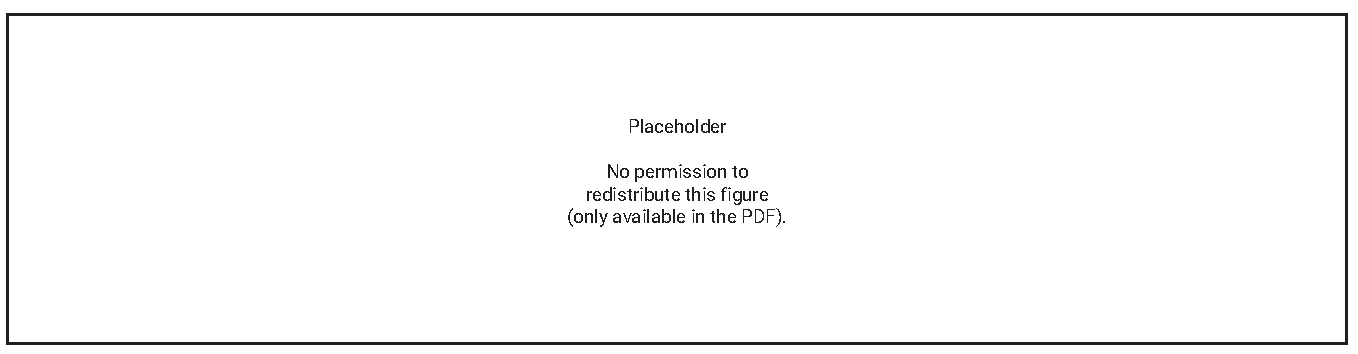
\includegraphics[width=1\textwidth]{diagram-labelsinside}
\sidecaption{\label{fig:labelsinside} Moving the labels inside objects reduces clutter. Note how the left-hand-side figure is centered in the left part of the figure to keep the figure balanced (reproduced from \cite{Carter12} with permission).}[-6\baselineskip]
\end{figure}

\begin{marginfigure}
\centering
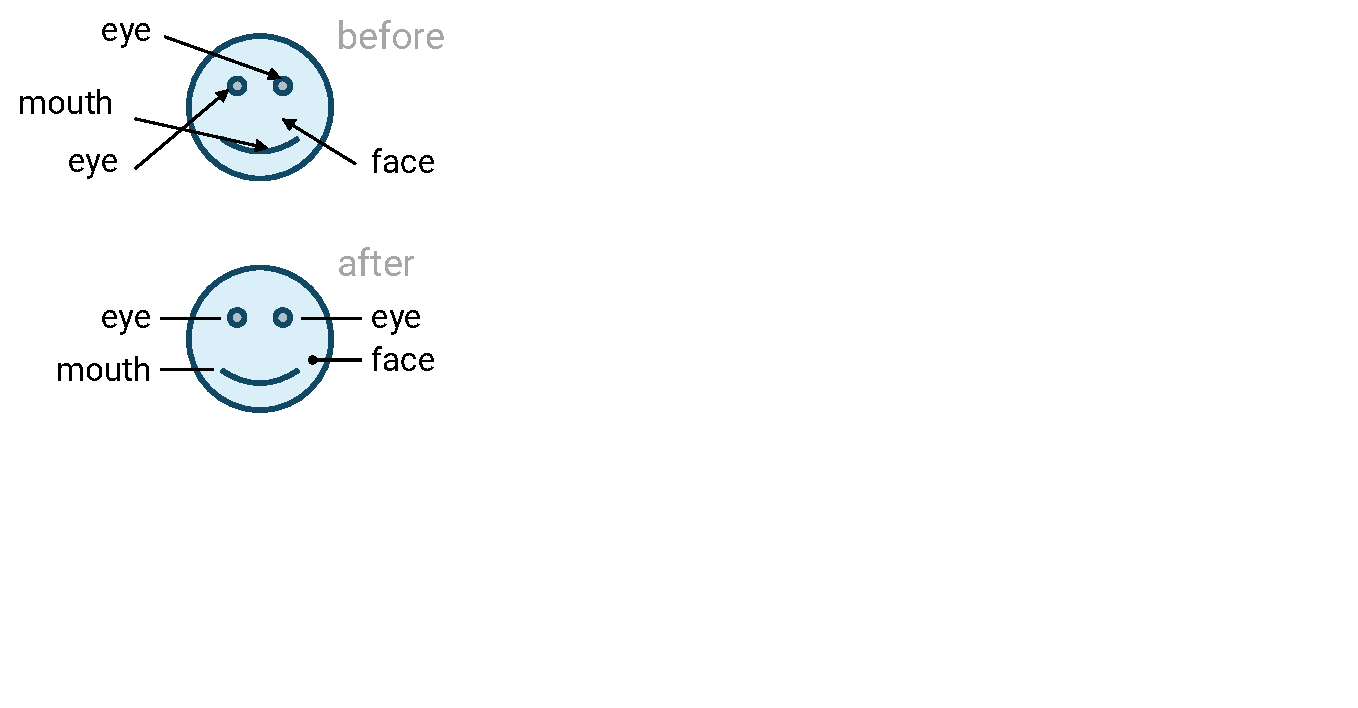
\includegraphics[width=1\textwidth]{diagram-labelsoutside}
\caption{\label{fig:labelsoutside} Outside labels should not distract the reader (own illustration, inspired by \cite{Carter12}).}%[-1\baselineskip]
\end{marginfigure}

Figure~\ref{fig:labelsoutside} illustrates critical principles when labels are \emph{outside} of a shape. First of all, keep the lines as short as possible (proximity). Consider removing the arrowheads from the lines that point into an object to avoid confusion with other arrows in the diagram. Also, avoid crossing lines. Align labels on the left-hand side of an object flush right and vice versa (symmetry). Aim for consistency by making the lines parallel. Keep adequate amounts of surrounding whitespace.

Diagrams that visualize structures can work fine with few labels. In contrast, diagrams that visualize procedures or more complex relationships need more textual explanation. Consider adding longer descriptions right next to the corresponding locations (proximity) as shown in Fig.~\ref{fig:explanations}.

\begin{figure}[t]
\centering

\includegraphics[width=1\textwidth]{diagram-explanations} 
\sidecaption{\label{fig:explanations} Complex diagrams benefit from integrated explanations. Source of figure as cited by \cite{Ware12}: R Chandler and J. Sweller (1991). Cognitive load theory and the format of instruction. \emph{Cognition and Instruction}, 8:4, 293–332, DOI: 10.1207/s1532690xci0804\_2, \url{www.tandfonline.com}. This figure is not subject to the Creative Commons License under which this guide is published (cf. Sect.~\ref{sec:license}); copyright is held by the publisher and/or the authors.}[-9\baselineskip]
\end{figure}


\subsection{Variations}

\begin{figure*}[t]
\centering
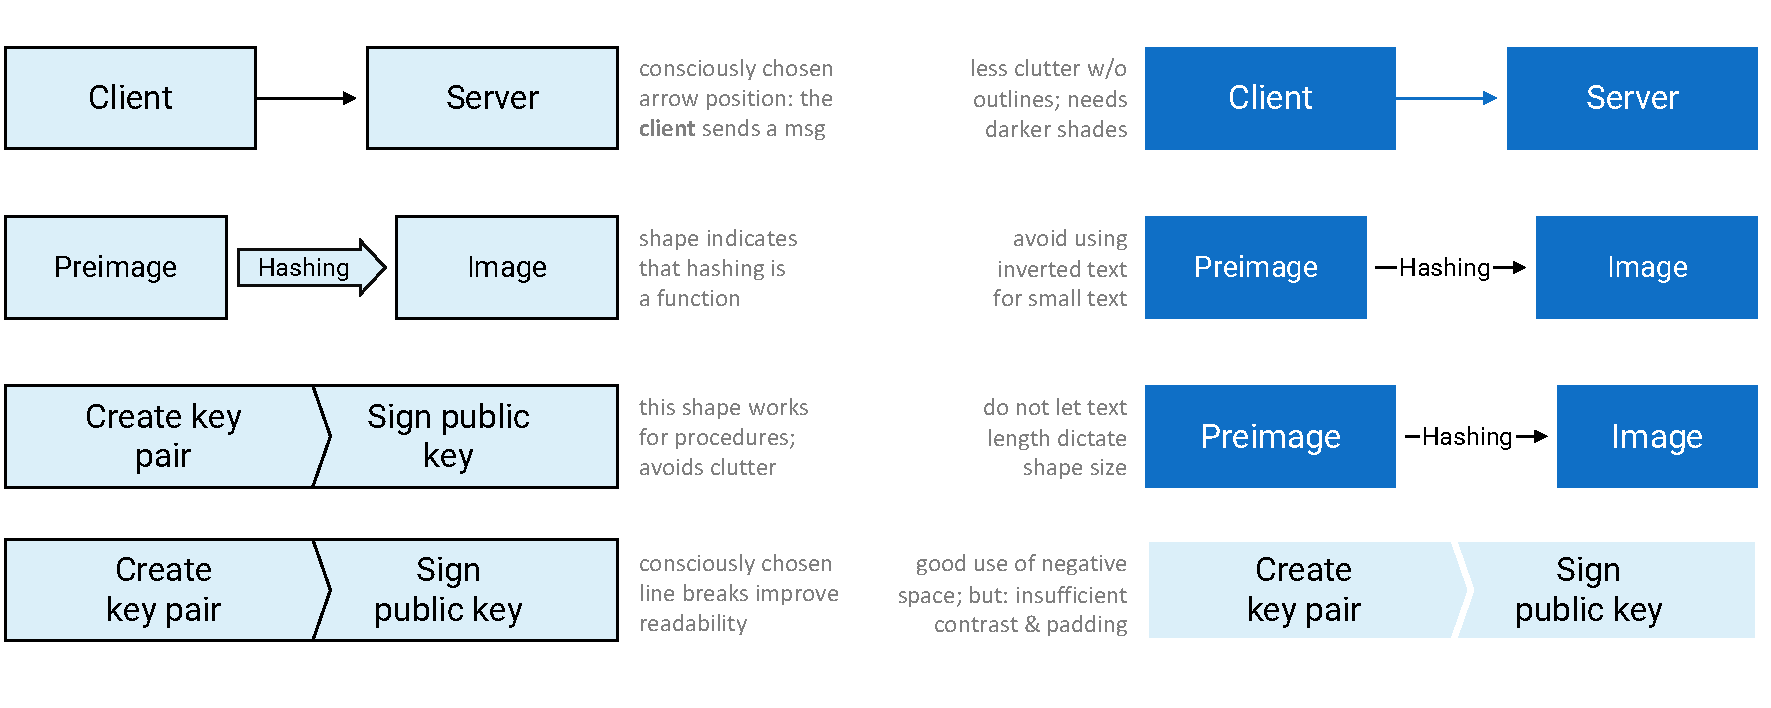
\includegraphics[width=1\widefigurewidth]{diagram-variations}
\sidecaption{\label{fig:diagvariations} Eight variations resulting from combining different outline, shade, and arrow styles.}[-1\baselineskip]
\end{figure*}

Common drawing tools provide a large number of shapes. What is missing, however, is guidance on how to combine them reasonably. Figure~\ref{fig:diagvariations} displays eight combinations.\sidenote{The advice in the following paragraphs has been compiled from \url{https://www.slideshare.net/otikik/how-to-make-awesome-diagrams-for-your-slides/19-Size_doesnt_mean_long_name}.}

The first variation in the left-hand column shows a style useful for depicting information exchange between systems, such as servers and clients. The second variation uses an arrow shape, which emphasizes the activity represented by the arrow. The third and fourth examples in the left-hand column depict two steps from a process without too much visual clutter. We prefer the latter one because the text wraps at sensible points.

The right-hand column shows variations without outlines. At first glance, this sounds like a good  idea: it avoids visual clutter (the outlines). Note, however, that shapes without outlines need more saturated and darker color to differentiate them from the background.  If the number of shapes in a diagram is large, this approach can make it more difficult to read the diagram because all shapes appear to be emphasized simultaneously.

If you use dark shapes, you should avoid having white text on dark background for small font sizes. As shown in the second variation on the right-hand side of Fig.~\ref{fig:diagvariations}, you will have to make changes to some shapes.

In any case, you should choose the sizes of shapes consciously. Represent objects with identical properties with shapes of the same size. If the labels do not fit into the shapes, you can either reduce the font size, put the labels next to the box, or increase the size of all shapes (by rearranging the diagram).

Finally, consider the option of using negative space, as shown in the bottom-right corner of Fig.~\ref{fig:diagvariations}. Again, this can be a useful means to avoid visual clutter. However, if you increase the width of the surrounding white stroke (as was done for the example figure), the (vertical) padding in the shape will become too narrow. Moreover, you cannot easily align such shapes with other shapes with thinner strokes.


\section{Graphs}

In this section, we review common design principles for graphs (also called charts or plots). Besides our guidelines, we will present the examples shown by Carter \cite{Carter12}.

The first step in data visualization is to \textbf{pick a reasonable chart type}. Most visualization needs that arise in a thesis can be addressed with line charts, bar charts, and histograms, and scatter plots. There are many more chart types such as Chord Diagrams, Sankey Diagrams, and the Nightingale Rose Chart.\sidenote{For comprehensive overviews and guidance see \url{https://datavizcatalogue.com}, \url{https://depictdatastudio.com/charts/}, \url{https://www.data-to-viz.com/img/poster/poster_big.png} and \url{https://www.labnol.org/images/2008/data-chart-type.png}.}
These and other advanced chart types \emph{can} be useful in particular situations. In general, however, we recommend sticking to more basic chart types. In particular, \textbf{avoid pie charts} unless you know what you are doing.

General advice for any graph is to have \textbf{legible axis labels} and, if more than one data series is visualized, a legend for the data series. Moreover, remember to use colors effectively (cf. Sect.~\ref{sec:color}).

The following sections provide more information on two essential chart types, line charts and bar charts. The recommendations are very concrete. You may find that you cannot follow all of them using your plotting tool of choice. If this limitation bothers you, consider editing the plotting tool's output with a vector drawing program such as Inkscape or Adobe Illustrator.

\subsection{Line Charts}

Line charts show how one variable (the one on the y-axis) changes when another one varies within a given range. Line charts are particularly useful to visualize time series.

Often, there are many lines to be plotted. Resist the temptation to add more than three lines into one line chart if the lines overlap. Instead, create multiple charts that have one of the lines in common. This line serves as a baseline, easing comparison.

Figure~\ref{fig:linecharts} summarizes Carter's advice on line charts.

\begin{figure*}[t]
\centering
%\vspace{3\baselineskip}

\includegraphics[width=1\widefigurewidth]{graphs-linecharts}
\sidecaption{\label{fig:linecharts} Advice for line charts (reproduced from \cite{Carter12} with permission). %Remark on the layout: As seen in this case, putting a wide figure below another one does not look very pleasing.
}[-1\baselineskip]
\end{figure*}

\subsection{Bar Charts}

The top row of Fig.~\ref{fig:barcharts} summarizes Carter's advice on bar charts.
Bar charts are useful to compare the value of a single variable under different circumstances. The value of the variable corresponds to the length of a bar. In principle, a single bar chart can also show the values of \emph{different} variables. Note, however, that such a chart is more challenging to read, especially when the variables need differently scaled Y-axes (one to the left and one to the right of the chart).

The bars can be drawn horizontally and vertically.\sidenote{See \url{https://depictdatastudio.com/when-to-use-horizontal-bar-charts-vs-vertical-column-charts/} for more guidance.} It is common to use vertical bars for time series (time on the x-axis). You can also use vertical bars if the values on the x-axis are on an ordinal scale (i.\,e., they are arranged in their natural order). Vertical bars do not work well with long labels. Rotating labels makes them challenging to read. On the other hand, horizontal bar charts work well with longer labels (align the labels flush right next to the bars).

The advice in this section assumes vertical bars. In vertical bar charts, the Y-axis corresponds to the value of the variable, and the X-axis is typically used for a categorial variable, which represents the different circumstances.

An advanced version of a classical bar chart is a stacked bar chart, an excellent alternative to visualize proportions of a whole. In contrast, to pie charts, which can be deceiving, stacked bar charts are more accurate and can be easily compared.

\begin{figure*}[t]
\centering
\vspace{4\baselineskip}
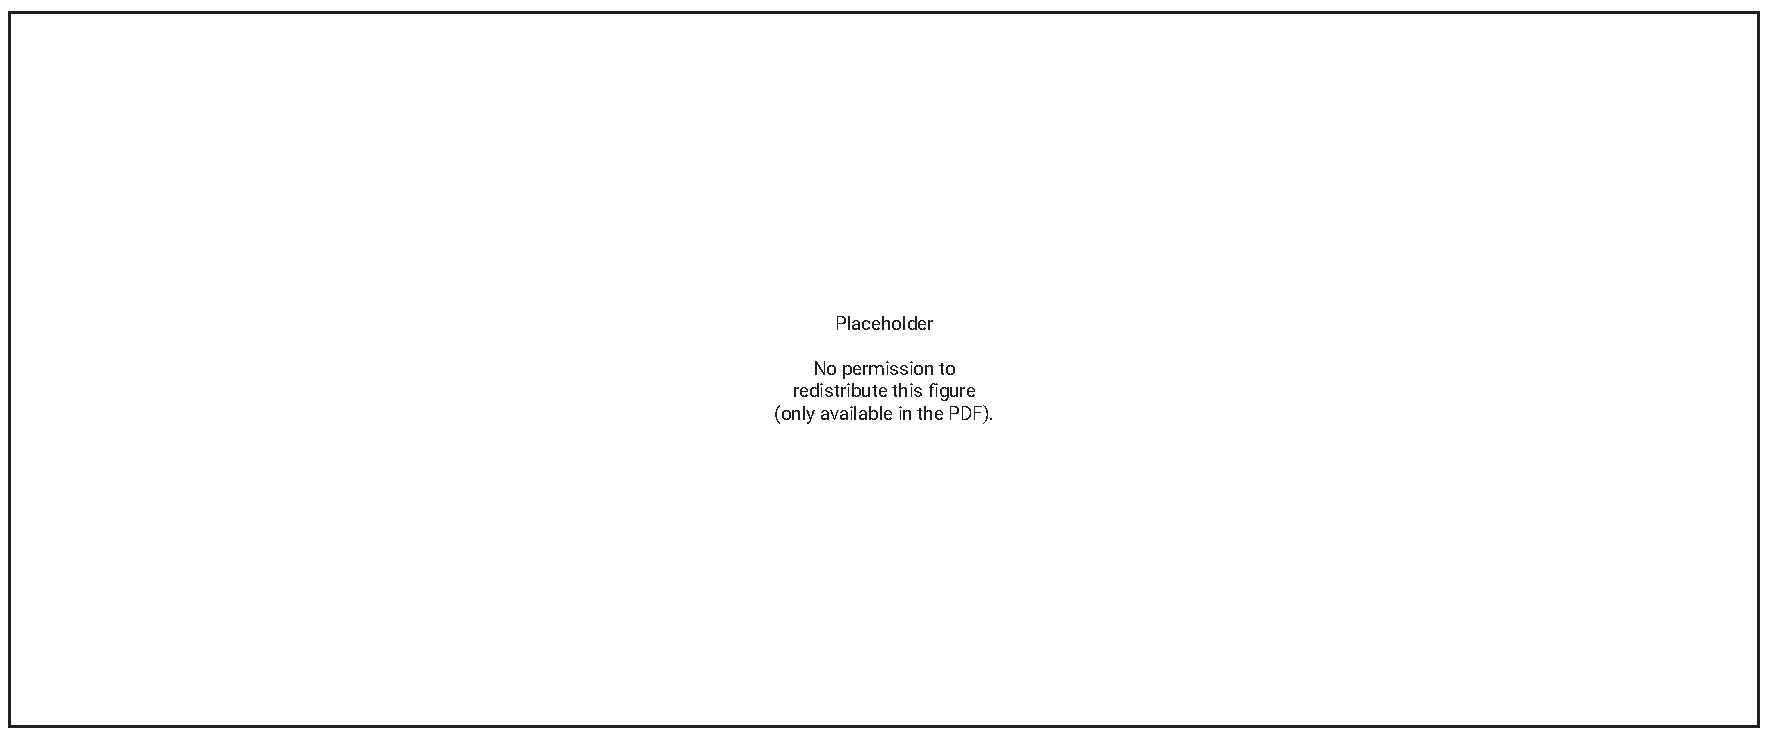
\includegraphics[width=1\widefigurewidth]{graphs-barcharts}

\bigskip

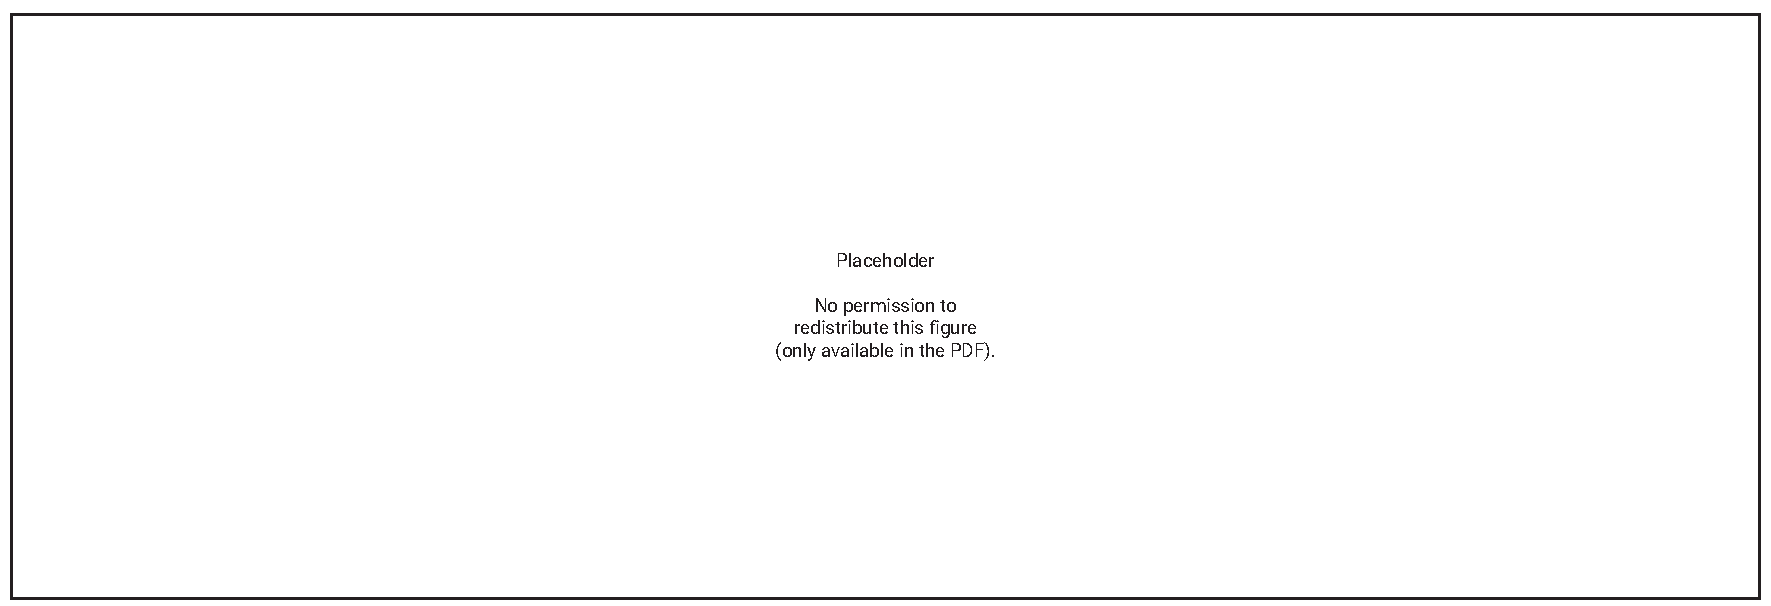
\includegraphics[width=1\widefigurewidth]{graphs-histograms}
\sidecaption{\label{fig:barcharts} Advice for bar charts and histograms (reproduced from \cite{Carter12} with permission).}
\end{figure*}

\paragraph{Histograms} A special kind of bar charts is a histogram. Carter gives a concise explanation of the purpose of a histogram: ``A histogram shows the distribution of data and the relative frequency with which the data occur. It essentially offers the audience an estimate of the probability distribution of a dataset'' \cite{Carter12}. The bottom row of Fig.~\ref{fig:barcharts} summarizes Carter's advice on histograms.

%\begin{figure*}[t]
%\centering
%\vspace{4\baselineskip}
%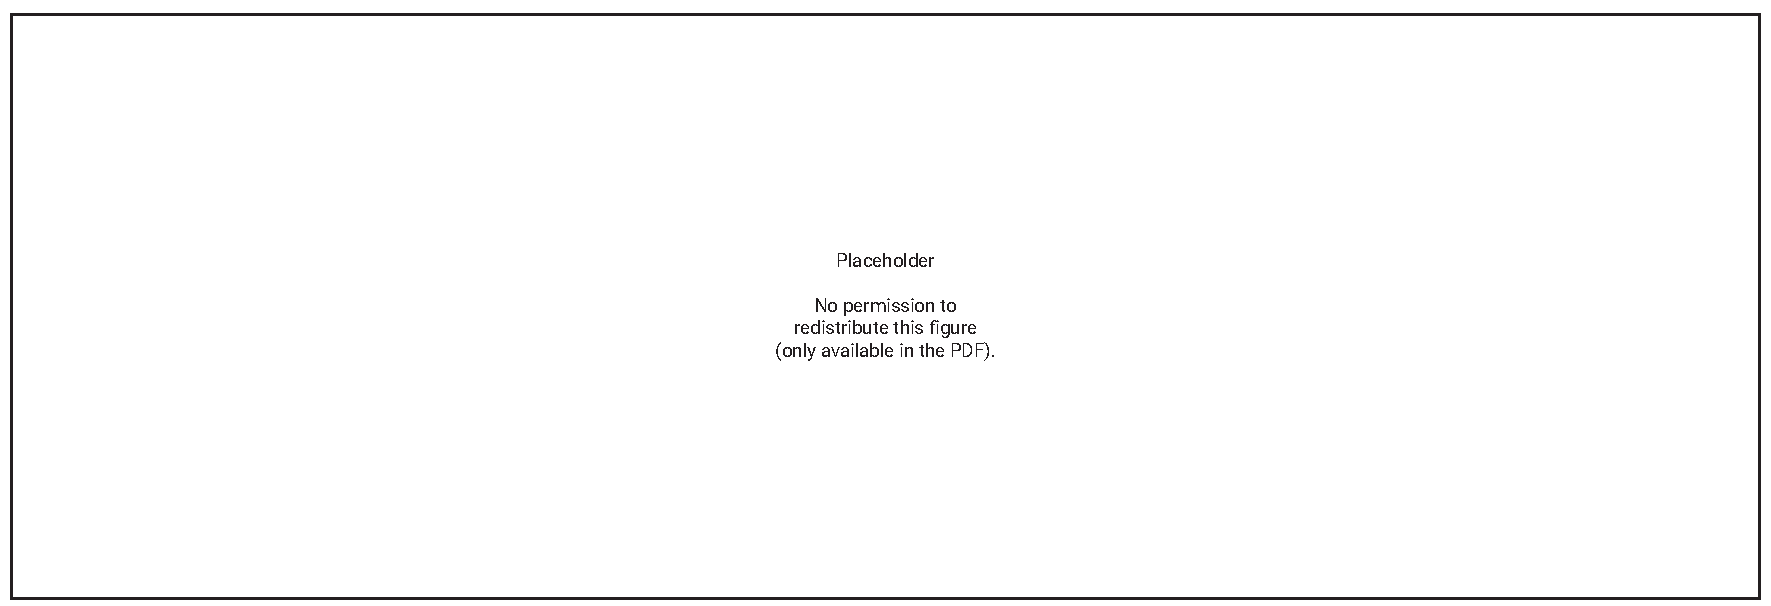
\includegraphics[width=1\widefigurewidth]{graphs-histograms}
%\sidecaption{\label{fig:histograms} Advice for histograms \cite{Carter12}.}
%\end{figure*}






\section{Tables}
\label{sec:tableguide}

Tables are useful to display multiple properties for several entities. This section summarizes Carter's guidelines for designing effective tables \cite{Carter12}. Moreover, you will see how to apply the principles of organizing information (cf. Sect.~\ref{sec:organizinginfo}).

Often, the properties of entities have different scales and units. Readers usually expect that rows correspond to entities, and columns correspond to properties. This organization makes it easier to compare entities in terms of individual properties by focusing on the values in particular columns. It is easy to spot exceptional cases if they are printed vertically and the eye can move downwards. The example in Table~\ref{tab:colrows} shows this effect with two tables that contain the same data.

\begin{table*}[tb]
  \caption{\label{tab:colrows} The table to the left is easier to read than the table to the right (reproduced from \cite{Carter12} with permission).}
  \centering
  \footnotesize % use smaller fontsize in the table
  {\renewcommand{\arraystretch}{1.1} % increase vertical space between rows
  \begin{tabularx}{0.45\linewidth}{@{}Xccr@{}} % @{} omits outer horizontal margins, the "X" column uses up all remaining available space 
    \toprule
    Lake & Area ($\mathrm{km}^2$) & Length (km) & Depth (m)\\
    \midrule
    Malawi & 30,044 & 579 & 706 \\
    Tanganyika & 32,893 & 676 & 1470 \\
    Victoria & 59,485 & 322 & 84\\
    \bottomrule
  \end{tabularx}
  \hspace{\fill}
  \begin{tabularx}{0.45\linewidth}{@{}Xccr@{}} % @{} omits outer horizontal margins, the "X" column uses up all remaining available space 
    \toprule
    Lake & Malawi & Tanganyika & Victoria\\
    \midrule
    Area ($\mathrm{km}^2$) & 30,044 & 32,893 & 59,485 \\
    Length (km) & 579 & 676 & 322 \\
    Depth (m) & 706 & 1470 & 84\\
    \bottomrule
  \end{tabularx}
  }
\end{table*}

Follow the Gestalt principle of Hierarchy when you display information that can be grouped. Often, there is more than one way how to group data. Make a conscious decision about how you organize the table. Different forms of organization emphasize different aspects. For instance, the table to the left in Table~\ref{tab:groups} emphasizes the comparison between men and women. In contrast, the table to the right highlights the differences between the years.

\begin{table*}[tb]
\caption{Number of men and women selected by NASA to be astronauts by year of selection (reproduced from \cite{Carter12} with permission).}
\label{tab:groups}
\centering
\footnotesize % use smaller fontsize in the table
{\renewcommand{\arraystretch}{1.1} % increase vertical space between rows
  \begin{tabularx}{0.53\linewidth}{@{}Xcccccc@{}} % @{} omits outer horizontal margins, the "X" column uses up all remaining available space 
  \toprule
  & \multicolumn{3}{c}{\tabhead{Men}} & \multicolumn{3}{c}{\tabhead{Women}} \\
  \cmidrule(lr){2-4} \cmidrule(l){5-7}
  & \tabhead{1980} & \tabhead{1990} & \tabhead{2000} & \tabhead{1980} & \tabhead{1990} & \tabhead{2000}\\
  \midrule
  Mission specialist & 9 & 12 & 7 & 2 & 4 & 3\\
  Pilot &              8 &  6 & 7 & 0 & 1 & 0\\
  \midrule
  Total &             17 & 18 & 14 & 2 & 5 & 3\\
  \bottomrule
  \end{tabularx}
\hspace{\fill}
  \begin{tabularx}{0.42\linewidth}{@{}Xcccccc@{}} % @{} omits outer horizontal margins, the "X" column uses up all remaining available space 
  \toprule
  & \multicolumn{2}{c}{\tabhead{1980}} & \multicolumn{2}{c}{\tabhead{1990}} & \multicolumn{2}{c}{\tabhead{2000}}\\
  \cmidrule(lr){2-3} \cmidrule(lr){4-5} \cmidrule(l){6-7}
  & \tabhead{M} & \tabhead{F} & \tabhead{M} & \tabhead{F} & \tabhead{M} & \tabhead{F}\\
  \midrule
  Mission specialist & 9 & 2 & 12 & 4 & 7 & 3\\
  Pilot &              8 & 0 &  6 & 1 & 7 & 0\\
  \midrule
  Total &             17 & 2 & 18 & 5 & 14 & 3\\
  \bottomrule
  \end{tabularx}
}
\end{table*}

Make a conscious decision on how to order the columns. Revisit the five hat racks design principle in Sect.~\ref{sec:fivehatracks}. If there is no logical ordering, e.\,g.,  from very generic properties to more specific ones, order the columns alphabetically. Usually, derived pieces of information, results, and insights are to the right of labels and descriptive pieces of information.

Choosing an adequate order also applies to rows. Instead of sorting the rows alphabetically based on their label in the first column, consider sorting them based on a particular column's value. The resulting order can improve legibility a lot (principle of \emph{continuity}). Note that sorting the table by a specific column puts some emphasis on that particular column. This principle is visualized in Table~\ref{tab:roworder}.

\begin{table*}[tb]
  \caption{\label{tab:roworder} Listing planets in order from the sun, in alphabetical order, and in descending order of diameter (reproduced from \cite{Carter12} with permission).}
  \centering
  \footnotesize % use smaller fontsize in the table
  {\renewcommand{\arraystretch}{1.1} % increase vertical space between rows
  \begin{tabularx}{0.3\linewidth}{@{}Xrr@{}} % @{} omits outer horizontal margins, the "X" column uses up all remaining available space 
    \toprule
    Planet & Diameter & Mass \\
    \midrule
    Mercury & 0.38 & 0.06 \\
    Venus & 0.95 & 0.82 \\
    Earth & 1.00 & 1.00 \\
    Mars & 0.53 & 0.11 \\
    Jupiter & 11.21 & 317.80 \\
    Saturn & 9.45 & 95.20 \\
    Uranus & 4.01 & 14.60 \\
    Neptune & 3.88 & 17.20 \\
    \bottomrule
  \end{tabularx}
  \hspace{\fill}
  \begin{tabularx}{0.3\linewidth}{@{}Xrr@{}} % @{} omits outer horizontal margins, the "X" column uses up all remaining available space 
    \toprule
    Planet & Diameter & Mass \\
    \midrule
    Earth & 1.00 & 1.00 \\
    Jupiter & 11.21 & 317.80 \\
    Mars & 0.53 & 0.11 \\
    Mercury & 0.38 & 0.06 \\
    Neptune & 3.88 & 17.20 \\
    Saturn & 9.45 & 95.20 \\
    Uranus & 4.01 & 14.60 \\
    Venus & 0.95 & 0.82 \\
    \bottomrule
  \end{tabularx}
  \hspace{\fill}
  \begin{tabularx}{0.3\linewidth}{@{}Xrr@{}} % @{} omits outer horizontal margins, the "X" column uses up all remaining available space 
    \toprule
    Planet & Diameter & Mass \\
    \midrule
    Jupiter & 11.21 & 317.80 \\
    Saturn & 9.45 & 95.20 \\
    Uranus & 4.01 & 14.60 \\
    Neptune & 3.88 & 17.20 \\
    Earth & 1.00 & 1.00 \\
    Venus & 0.95 & 0.82 \\
    Mars & 0.53 & 0.11 \\
    Mercury & 0.38 & 0.06 \\
    \bottomrule
  \end{tabularx}
  }
\end{table*}